\documentclass[final,t]{beamer}
\catcode`\@=11
\mode<presentation>
{
%  \usetheme{Warsaw}
%  \usetheme{Aachen}
%  \usetheme{Oldi6}
%  \usetheme{I6td}
  \usetheme{I6dv}
%  \usetheme{I6pd}
%  \usetheme{I6pd2}
}



\def\bold#1{\mbox {\bf #1}}\def \vc #1#2{\bold {#1}_{#2}}\def \bftil #1#2{\bold {\widetild #1}_{#2}}
\def\bea{ \begin{eqnarray}}
\def\eea{\end{eqnarray}}
\def\cref#1{(\ref {#1})}
\def\Let@{\relax\iffalse{\fi\let\\=\cr\iffalse}\fi}
\def\vspace@{\def\vspace##1{\noalign{\vskip##1 }}}
\def\mat{\left[\matrix} \def\endmat{\endmatrix\right]}
%\def\vspace@{\def\vspace##1{\noalign{\vskip##1 }}}
\def\matrix{\,\vcenter\bgroup\Let@\vspace@
    \normalbaselines
  \m@th\ialign\bgroup\hfil$##$\hfil&&\quad\hfil$##$\hfil\crcr
    \mathstrut\crcr\noalign{\kern-\baselineskip}}
\def\endmatrix{\crcr\mathstrut\crcr\noalign{\kern-\baselineskip}\egroup
\egroup\,}


% additional settings
\setbeamerfont{itemize}{size=\normalsize}
\setbeamerfont{itemize/enumerate body}{size=\normalsize}
\setbeamerfont{itemize/enumerate subbody}{size=\normalsize}

% additional packages
\usepackage{times}
\usepackage{amsmath,amsthm, amssymb, latexsym,epsfig}
\usepackage{exscale}
%\boldmath
\usepackage{booktabs, array}
%\usepackage{rotating} %sideways environment
\usepackage[english]{babel}
\usepackage[utf8]{inputenc}
\usepackage{natbib}
\usepackage{ragged2e}

\usepackage{subfigure}
\usepackage[orientation=landscape,size=custom,width=90,height=120,scale=1.15]{beamerposter}

\listfiles
\graphicspath{{figures/}}
% Display a grid to help align images
%\beamertemplategridbackground[1cm]



\title{\huge One century of data from Vassouras Magnetic Observatory (1915-2015)}


\author[Benevides, Bassrei]{Artur Benevides, Edwin Camacho*, Vitor Silveira, Israelli Rodrigo, Rodrigo Melhorato e Kátia Pinheiro}
\institute[ON-MCTIC]{Observatório Nacional}
\date[Nov , 2017]{Nov. 15 , 2017}


% abbreviations
\usepackage{xspace}
\makeatletter
\DeclareRobustCommand\onedot{\futurelet\@let@token\@onedot}
\def\@onedot{\ifx\@let@token.\else.\null\fi\xspace}
\def\eg{{e.g}\onedot} \def\Eg{{E.g}\onedot}
\def\ie{{i.e}\onedot} \def\Ie{{I.e}\onedot}
\def\cf{{c.f}\onedot} \def\Cf{{C.f}\onedot}
\def\etc{{etc}\onedot}
\def\vs{{vs}\onedot}
\def\wrt{w.r.t\onedot}
\def\dof{d.o.f\onedot}
\def\etal{{et al}\onedot}
\makeatother

%%%%%%%%%%%%%%%%%%%%%%%%%%%%%%%%%%%%%%%%%%%%%%%%%%%%%%%%%%%%%%%%%%%%%%%%%%%%%%%%%%%%%%%%%%%%%%%%%%%%%%%%%%%%
%%%%%%%%%%%%%%%%%%%%%%%%%%%%%%%%%%%%%%%%%%%%%%%%%%%%%%%%%%%%%%%%%%%%%%%%%%%%%%%%%%%%%%%%%%%%%%%%%%%%%%%%%%%%
\begin{document}

  \begin{columns}[t]
    \begin{column}{.66\linewidth}

%%%%%%%%%%%%%%%%%%%%%%%%%%%%%%%%%%%%%%%%%%%%%%%%%%%%%%%%%%%%%%%%%%%%%%%%%%%%%%%%%%%%%%%%%%%%%%%%%%%%%%%%%%%%
%%%%%%%%%%%%%%%%%%%%%%%%%%%%%%%%%% Primeira coluna %%%%%%%%%%%%%%%%%%%%%%%%%%%%%%%%%%%%%%%%%%%%%%%%%%%%%%%%%
%%%%%%%%%%%%%%%%%%%%%%%%%%%%%%%%%%%%%%%%%%%%%%%%%%%%%%%%%%%%%%%%%%%%%%%%%%%%%%%%%%%%%%%%%%%%%%%%%%%%%%%%%%%%
\begin{block}{Introduction}
\justifying	
 Vassouras Magnetic Observatory (VSS) was the first observatory in Brazil, starting its measurements in 1915. VSS plays an important role in monitoring of the magnetic field in the south hemisphere mainly because is located in region of Southern Atlantic Magnetic Anomaly (SAMA). VSS is part of the INTERMAGNET since 1999 because of its high data quality and transmission in real time.
 
 This work presents the history of VSS as well as the centennial dataset (1915-2015). We	explore the comparison of VSS data and results of IGRF model, present a day Solarquiet and storm data as well the main characteristics of the secular variation in	VSS and the possible geomagnetic jerks occurring in this period.	
		

	
\end{block}

\begin{block}{History (1915 - 2015)}
	
In 1913 the engineer and director of the Observatório Nacional (ON), Henrique Charles Morize in partnership with the astronomer Alix Correa Lemos idealized the the city of Vassouras, RJ (Latitude 22.4° S and 43.35° W) as the ideal place for installation of the VSS.
	
	
	
\end{block}


\begin{columns}
	\begin{column}{.31\linewidth}
	
\begin{block}{Theorical Fundamentals}

\begin{itemize}
	\justifying
	
\begin{itemize}
	\justifying
	\item \bf{Elements of the geomagnetic field}
\end{itemize}	
\[ F^{2} = X^{2} + Y^{2} + Z^{2},\]
 \[  H^{2} = X^{2} + Y^{2}, \]
\[	   X = Hcos(D),\]
\[	   Y = Hsen(D),\]
\[	   Z = Fsen(I),\]
\[	   H = Fcos(I).\]
   	
	
	\item \bf{Secular variation}
\end{itemize}
The secular variation is the sucessive difference of the values of field components given by:
\[\frac{dX}{dt} = X(t+1)-X(t)\]

where t represents time in years.

\begin{itemize}
\justifying
		\item \bf{Least Square Method (LSM)}
\end{itemize}

\begin{itemize}
\justifying
		\item \bf{Fit by spline interpolation}
\end{itemize}
The secular variation of X,Y and Z compontents were fitted using an algorithm  of linear fit by spline method: 
	\[ f(x)= f(x_{n-1})+t_{n-1}(x-x_{n-1}), \\
	for x_{n-1} \le x \le x_{n} \]\\

\begin{itemize}
\justifying
		\item \bf{Root Means Square (RMS)}
\end{itemize}
We calculated the erro between the model IGRF and the data from VSS using RMS:
\[e_{RMS}=\frac{1}{N} \sqrt{\sum\limits_{i=1}^{N}(m_{i}-d_{i})^{2}}, 
\]
the RMS can be view in the legends of figures.
 
	
\end{block}	

\begin{block}{Geomagnetic Field Elements}

Evolution of the main field components,. From 1915 until 1999 the  annual means data  were given directly by VSS, from 1990 until 2015 was perform annual means using data of minute of the components from INTERMAGNET.

\begin{figure}
\centering
\includegraphics[width=0.9\linewidth, height=0.1\textheight]{"figs_ed/X mean all_V2"}
\caption[1]{1}
\label{fig:Xmeanall_V2}
\end{figure}
   
\begin{figure}
\centering
\includegraphics[width=0.9\linewidth, height=0.1\textheight]{"figs_ed/Y mean all_v2"}
\caption{2}

\label{fig:Ymeanall_v2}
\end{figure}


\end{block}

\end{column}
%%%%%%%%%%%%%%%%%%%%%%%%%%%%%%%%%%%%%%%%%%%%%%%%%%%%%%%%%%%%%%%%%%%%%%%%%%%%%%%%%%%%%%%%%%%%%%%%%%%%%%%%%%%%%%%%%%%

\begin{column}{.31\linewidth}

\begin{block}{Geomagnetic Field Elements}
	
\begin{figure}
\centering
\includegraphics[width=0.8\linewidth, height=0.1\textheight]{"figs_ed/Z mean all_v2"}
\caption{3}
\label{fig:Zmeanall_v2}
\end{figure}

\begin{figure}
\centering
\includegraphics[width=0.8\linewidth, height=0.1\textheight]{"figs_ed/F mean all_v2"}
\caption{4}
\label{fig:Fmeanall_v2}
\end{figure}

\begin{figure}
	\centering
	\includegraphics[width=0.8\linewidth, height=0.1\textheight]{"figs_ed/H mean all_v2"}
	\caption{5}
	\label{fig:Hmeanall_v2}
\end{figure}


\begin{figure}
\centering
\includegraphics[width=0.9\linewidth, height=0.1\textheight]{"figs_ed/D mean all_v2"}
\caption{6}
\label{fig:Dmeanall_v2}
\end{figure}


\begin{figure}
\centering
\includegraphics[width=0.9\linewidth, height=0.1\textheight]{"figs_ed/I mean all_v2"}
\caption{7}
\label{fig:Imeanall_v2}
\end{figure}


	
	
\end{block}



\begin{block}{Sq and Storm Days}
	\justifying
\begin{figure}
\centering
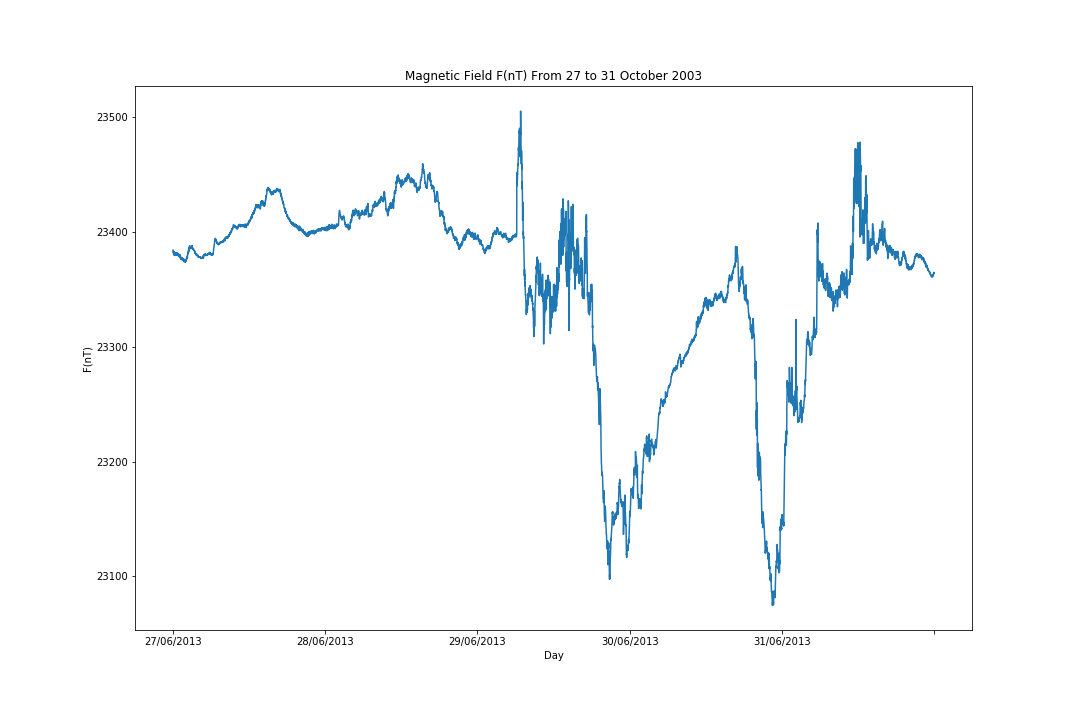
\includegraphics[width=0.8\linewidth]{F27_31_october(2003)}
\label{fig:F27_31_october(2003)}
\end{figure}
	
	
\end{block}	
	

\end{column}


\begin{column}{.31\linewidth}
	
	
	\begin{block}{Geomagnetics Jerks}
		\justifying
		Possible ocurrence of geomagnetic jerks.
		Secular variation is loosely used to indicate slow changes with time of the geomagnetic field
		(often found in the Y, X and Z componentS ) that are (probably) due to the changing pattern of core
		flow:
		Analyzing directly the X, Y and Z components using LSM to fit trends: 	
		\begin{figure}
			\centering
			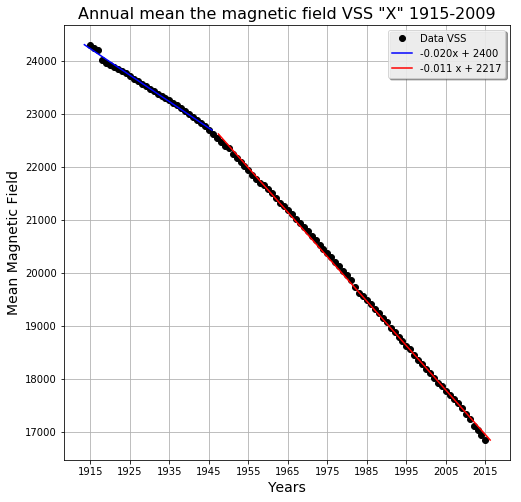
\includegraphics[width=0.5\linewidth]{retasX}
			\caption{9.}
			\label{w}
		\end{figure}	
		
		\begin{figure}
			\centering
			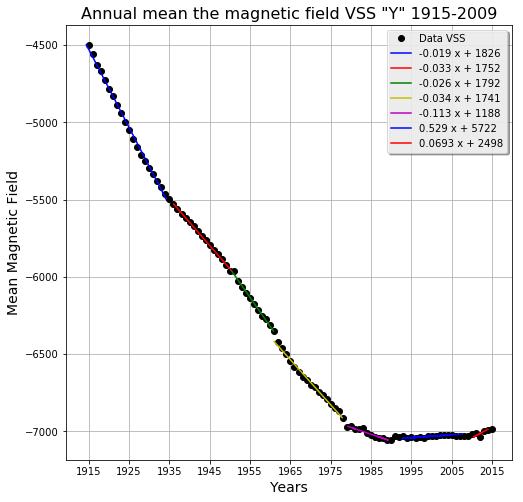
\includegraphics[width=0.5\linewidth]{retasY}
			\caption{10.}
			\label{fintetico}
		\end{figure}	
		
		
		\begin{figure}
			\centering
			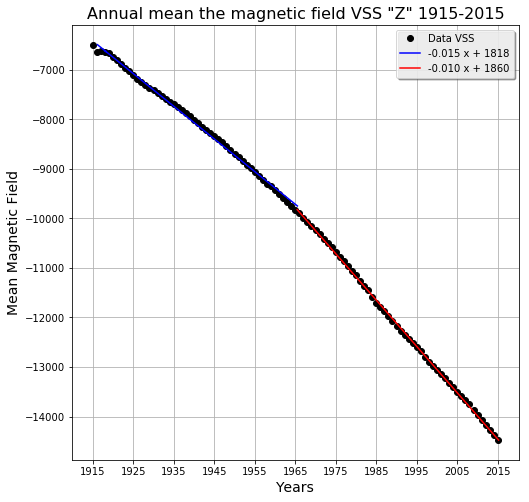
\includegraphics[width=0.5\linewidth]{retasZ}
			\caption{11.}
			\label{fig:g_Sintetico}
		\end{figure}

Analyzing the secular variations (dX/dt, dY/dt e dZ/dt) by spline fits: 		
		\begin{figure}
			\centering
			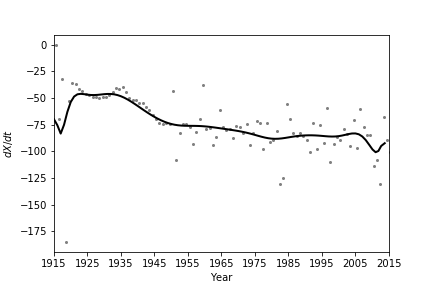
\includegraphics[width=0.7\linewidth]{spline101sv_X_spline}
			\caption{12. Secular variation to X component}
			\label{SPLINEx}
		\end{figure}
		
		\begin{figure}
			\centering
			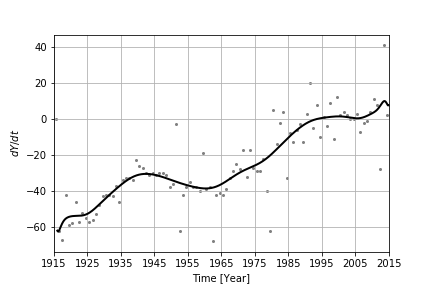
\includegraphics[width=0.7\linewidth]{spline100sv_y_spline}
			\caption{13. Secular variation to Y component.}
			\label{SPLINEy}
		\end{figure}
		
		\begin{figure}
			\centering
			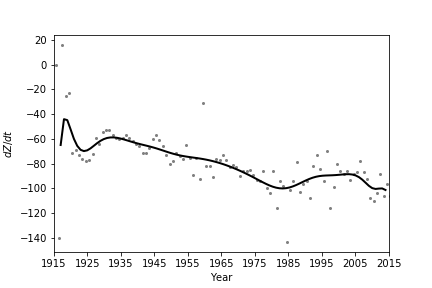
\includegraphics[width=0.7\linewidth]{spline100sv_z_spline}
			\caption{14 Secular variation to Z component.}
			\label{Splinez}
		\end{figure}
		
		
		
		
		
		
	\end{block}
\end{column}	

\end{columns}

\end{column}
%%%%%%%%%%%%%%%%%%%%%%%%%%%%%%%%%%%%%%%%%%%%%%%%%%%%%%%%%%%%%%%%%%%%%%%%%%%%%%%%%%%%%%%%%%%%%%%%%%%%%%%%%%%%
%%%%%%%%%%%%			Terceira Coluna %%%%%%%%%%%%%%%%%%%%%%%%%%%%%%%%%%%%%%%%%%%%%%%%%%%%%%%%%%%%%%%%%%%% %%%%%%%%%%%%							%%%%%%%%%%%%%%%%%%%%%%%%%%%%%%%%%%%%%%%%%%%%%%%%%%%%%%%%%%%%%%%%%%%%
%%%%%%%%%%%%%%%%%%%%%%%%%%%%%%%%%%%%%%%%%%%%%%%%%%%%%%%%%%%%%%%%%%%%%%%%%%%%%%%%%%%%%%%%%%%%%%%%%%%%%%%%%%%%
\begin{column}{.33\linewidth}


\begin{block}{VSS}
	\justifying
\begin{figure}
\centering
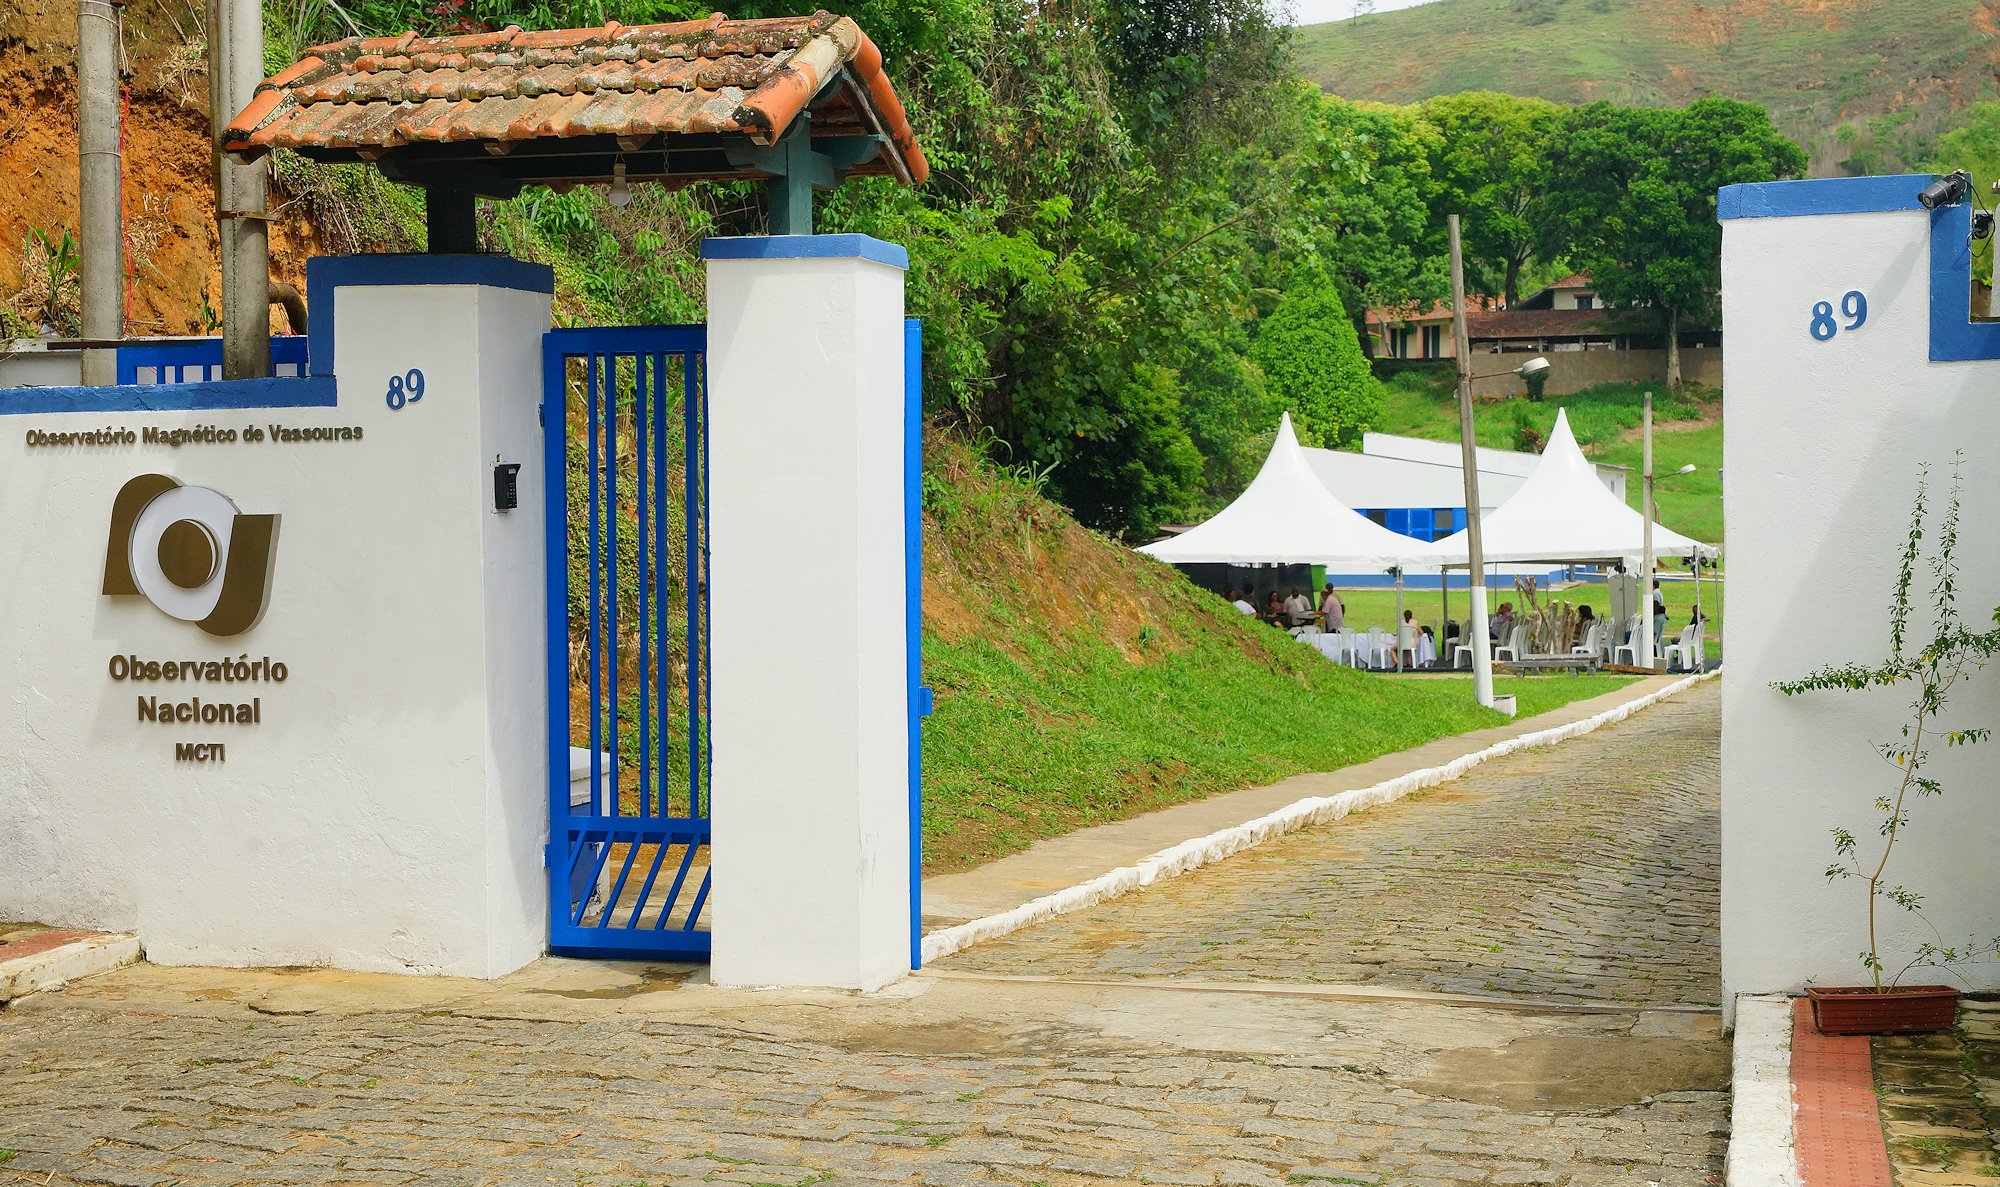
\includegraphics[width=0.8\linewidth]{OMV_JOELSONMOREIRA}
\caption{}
\label{fig:OMV_JOELSONMOREIRA}
\end{figure}





\end{block}


\begin{block}{VSS}
\centering

	 Period |\hspace{2.0cm}  Instruments   \\ 
	 
	 1915 - 1982 | "Ruska Observatory Pattern (Declination), QHM 534 (Horizontal component) and Earth Inductor Toepfer (Inclination) Variometer unifilar Toepfer 
	 
	 1982 - 2012 | DI-flux Bartington, MAG-01 with theodolite Zeiss 010 (1") (Declination and Inclination), PPM Geometrics 816 (Total intensity F).
	 
	 2012 - 2014 | Variometer fluxgate (INTERMAGNET)


\\

\begin{table}
\begin{tabular}{|c|c|c|c|}
		\hline
		\multicolumn{4}{|c|}{\textbf{Change/year}}\\	
	\hline   & VSS (nT)& IGRF12 (nT) & WMM2015 (nT)\\ 
	\hline Total intensity & -22,7  & -3.0  & -7.8  \\ 
	\hline X component & -74,7 & -98.0 & -93.3 \\ 
	\hline Y component & 24,9  & 2.2 & 5.4 \\ 
	\hline Z component & -79,8 & -91.6  & -94.1\\ 
	\hline H component  & -64,7 & -85.3 & -88.2\\ 
	\hline I component  & $-0° 14' 13"$ & $-0° 19' 15"$ &$-0° 19' 5"$\\ 
	\hline D component  & $-0° 7' 2,28"$ & $-0° 6' 25"$ &$ -0° 5' 59"$\\ 
	\hline 
\end{tabular} 
\caption{2. }
\end{table}		
\end{block}


%\begin{block}{References}
%\bibliographystyle{seg} 
%\bibliography{references}
%\end{block}



\begin{block}{References}

\begin{itemize}
\item
\end{itemize}
\vspace{-0.2cm}
\end{block}

\end{column}

\end{columns}
\end{document}


%\begin{figure}
%%	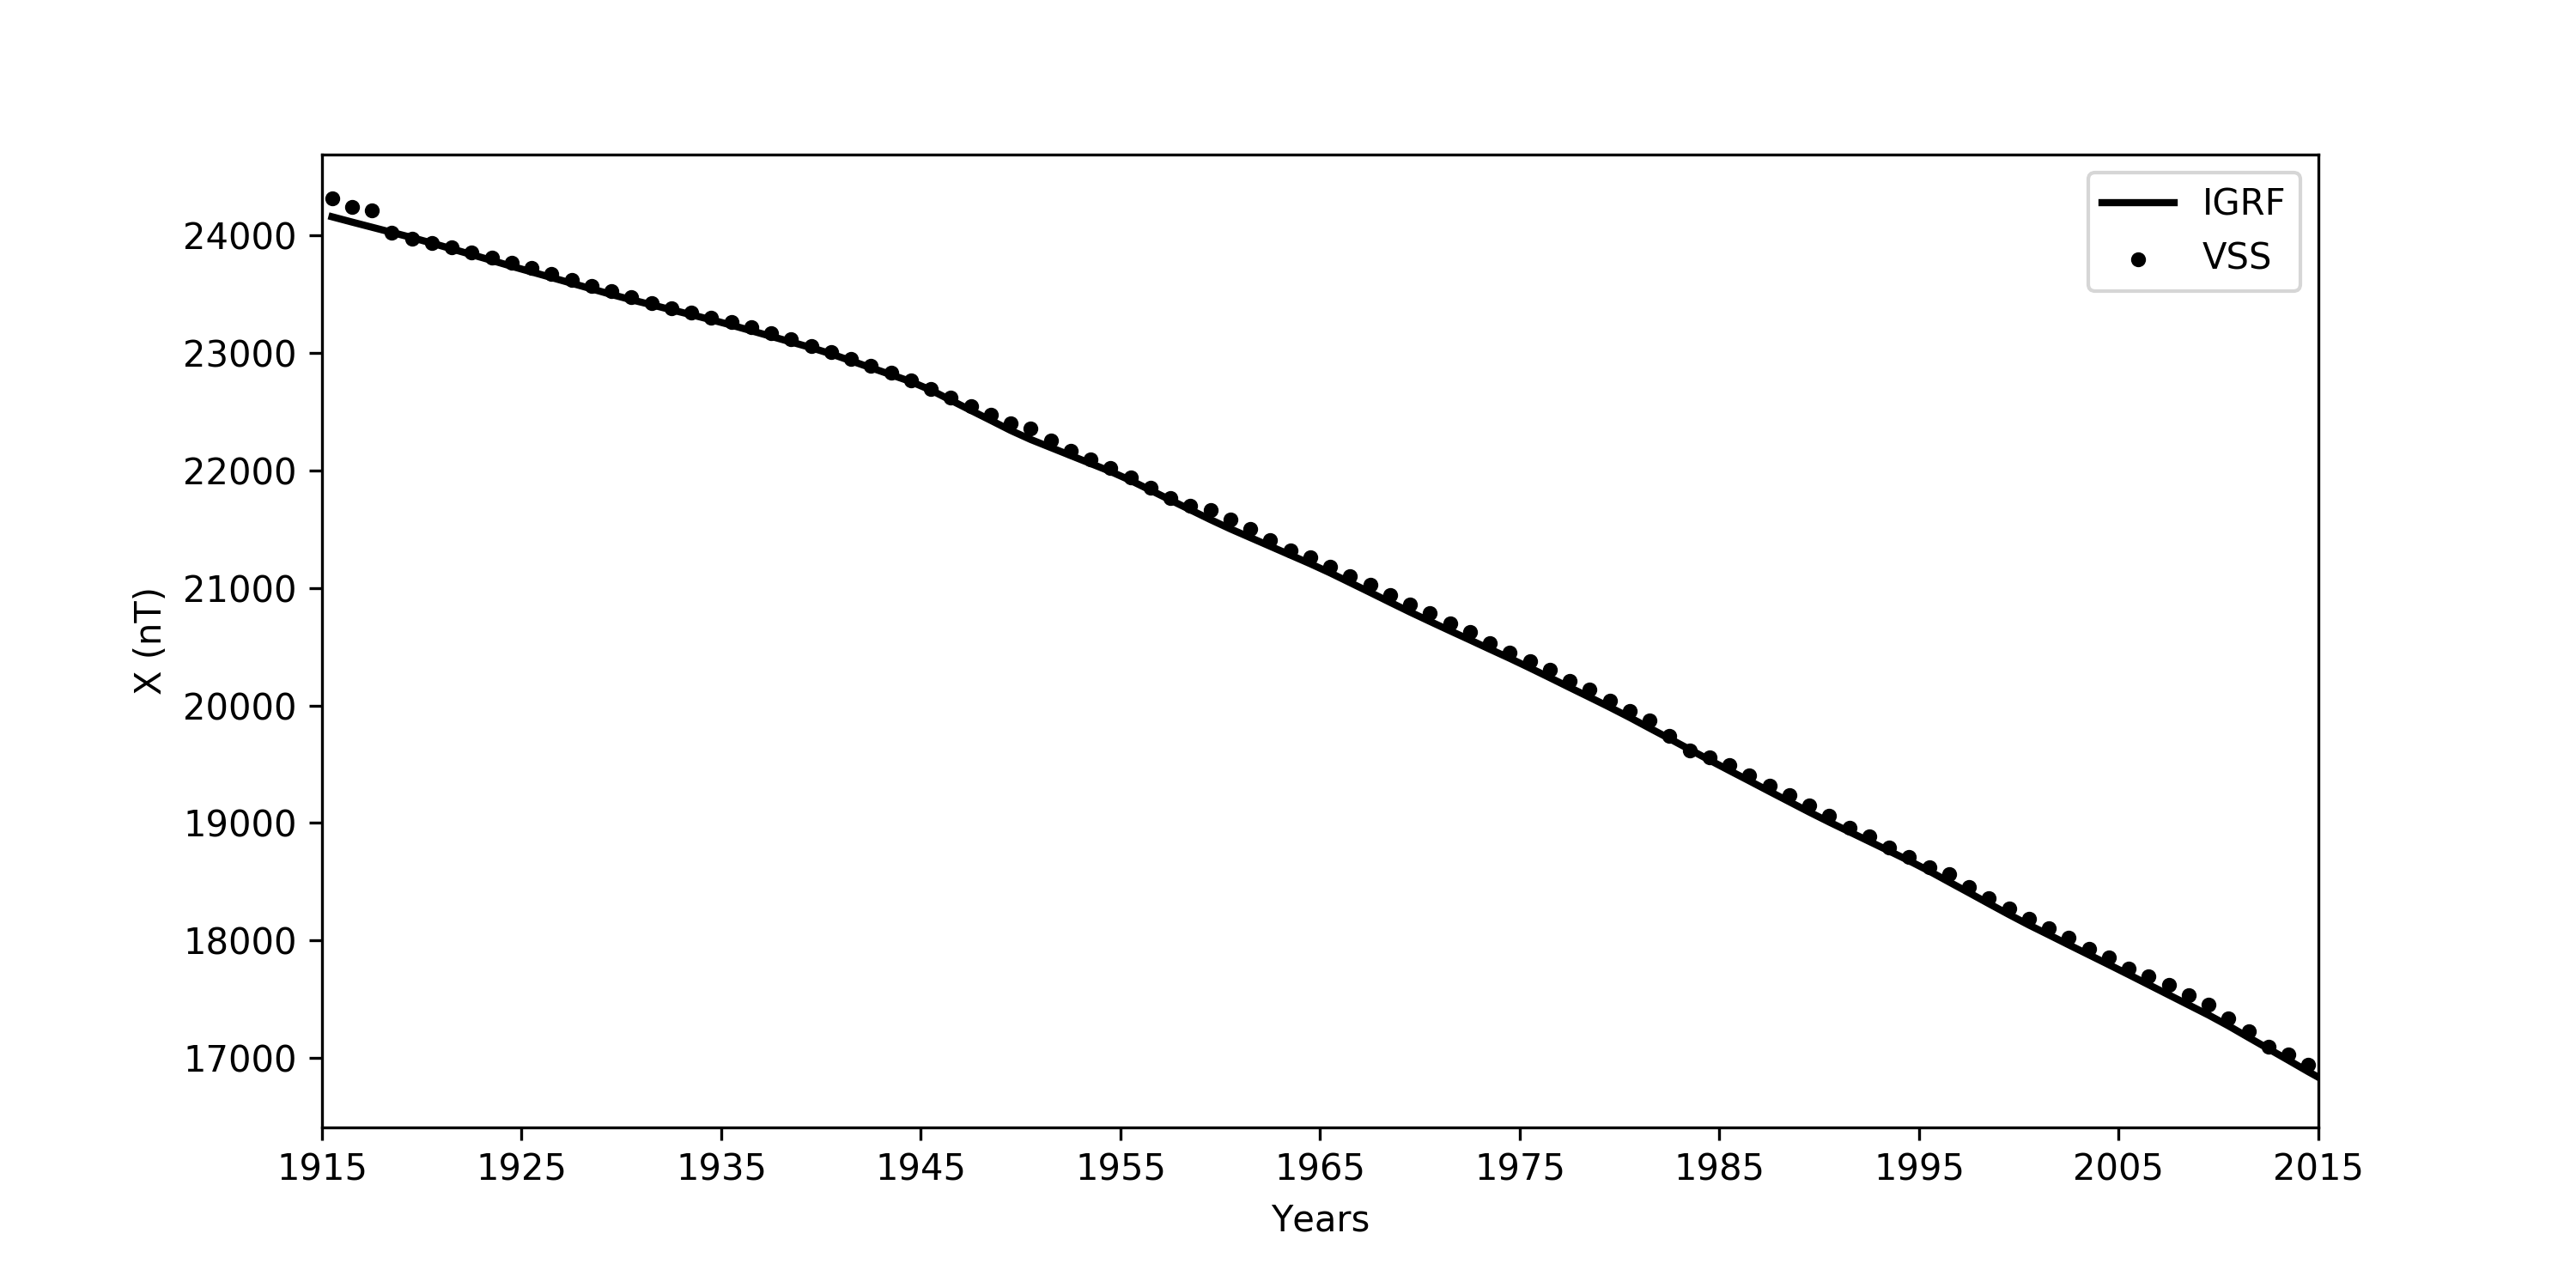
\includegraphics[width=1.0\linewidth]{X}
%	\caption{1. Root means square (RMS) between VSS data and IGRF model (X component) is 0.25 (\%)}
%	\label{X}
%\end{figure}

%\begin{figure}
%	\centering
%	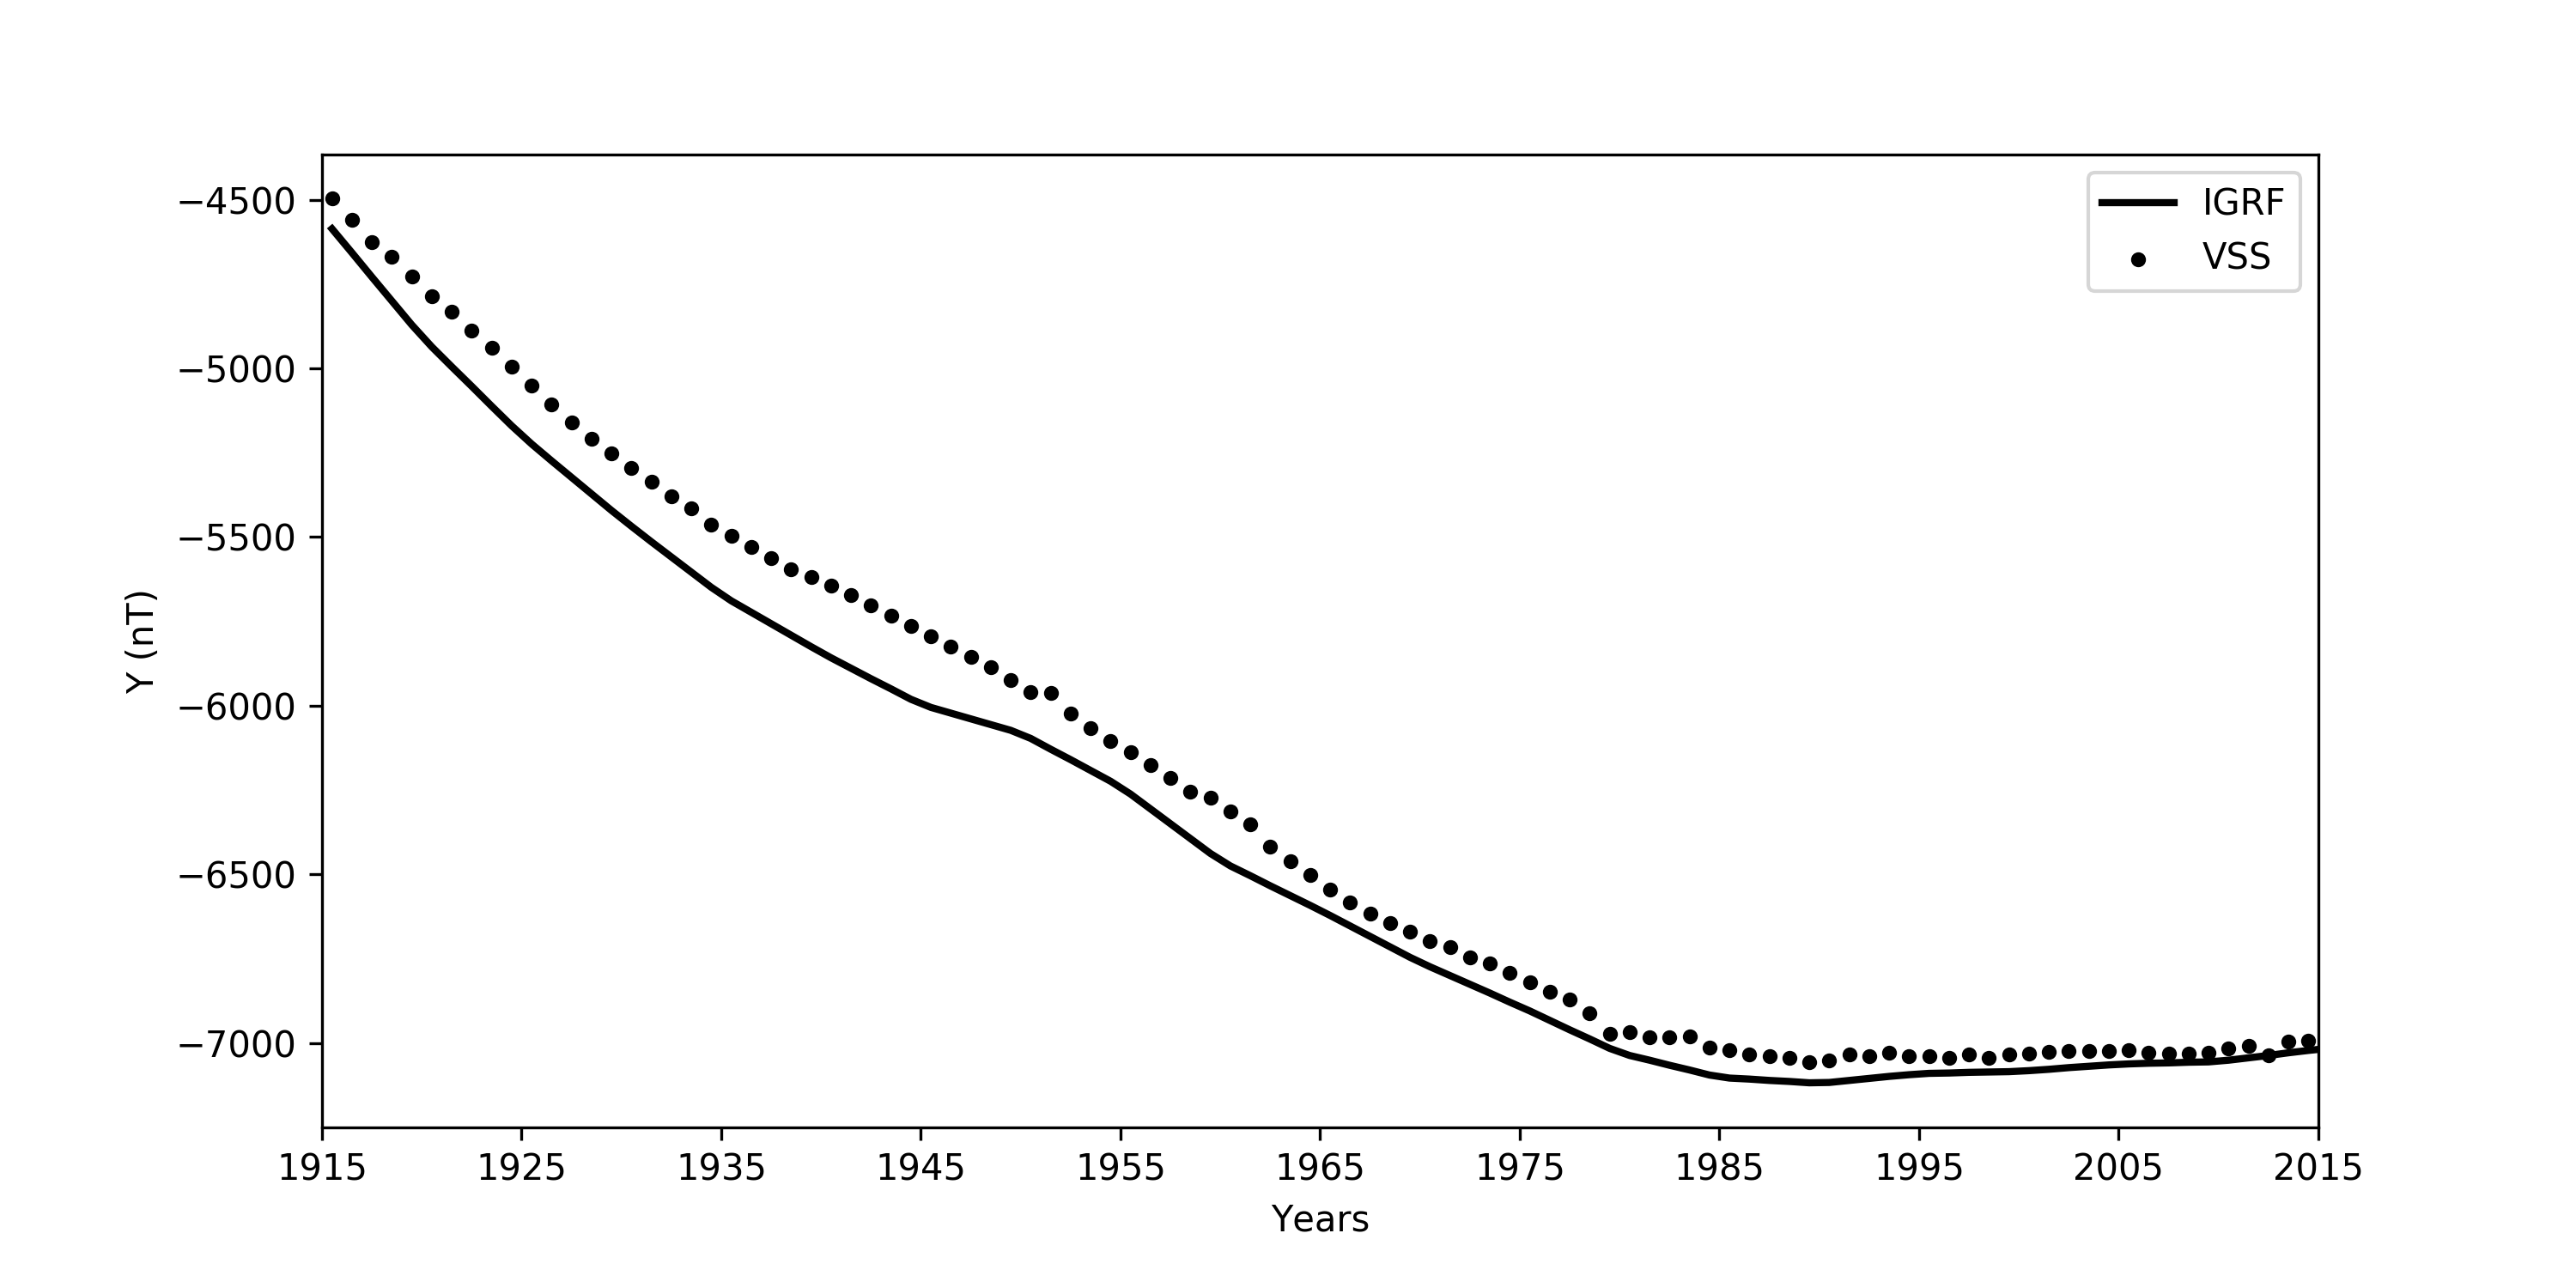
\includegraphics[width=1.0\linewidth]{Y}
%	\caption{2. RMS (Y component) = 1.98 (\%)}
%	\label{y}
%\end{figure}

%\begin{figure}
%	\centering
%	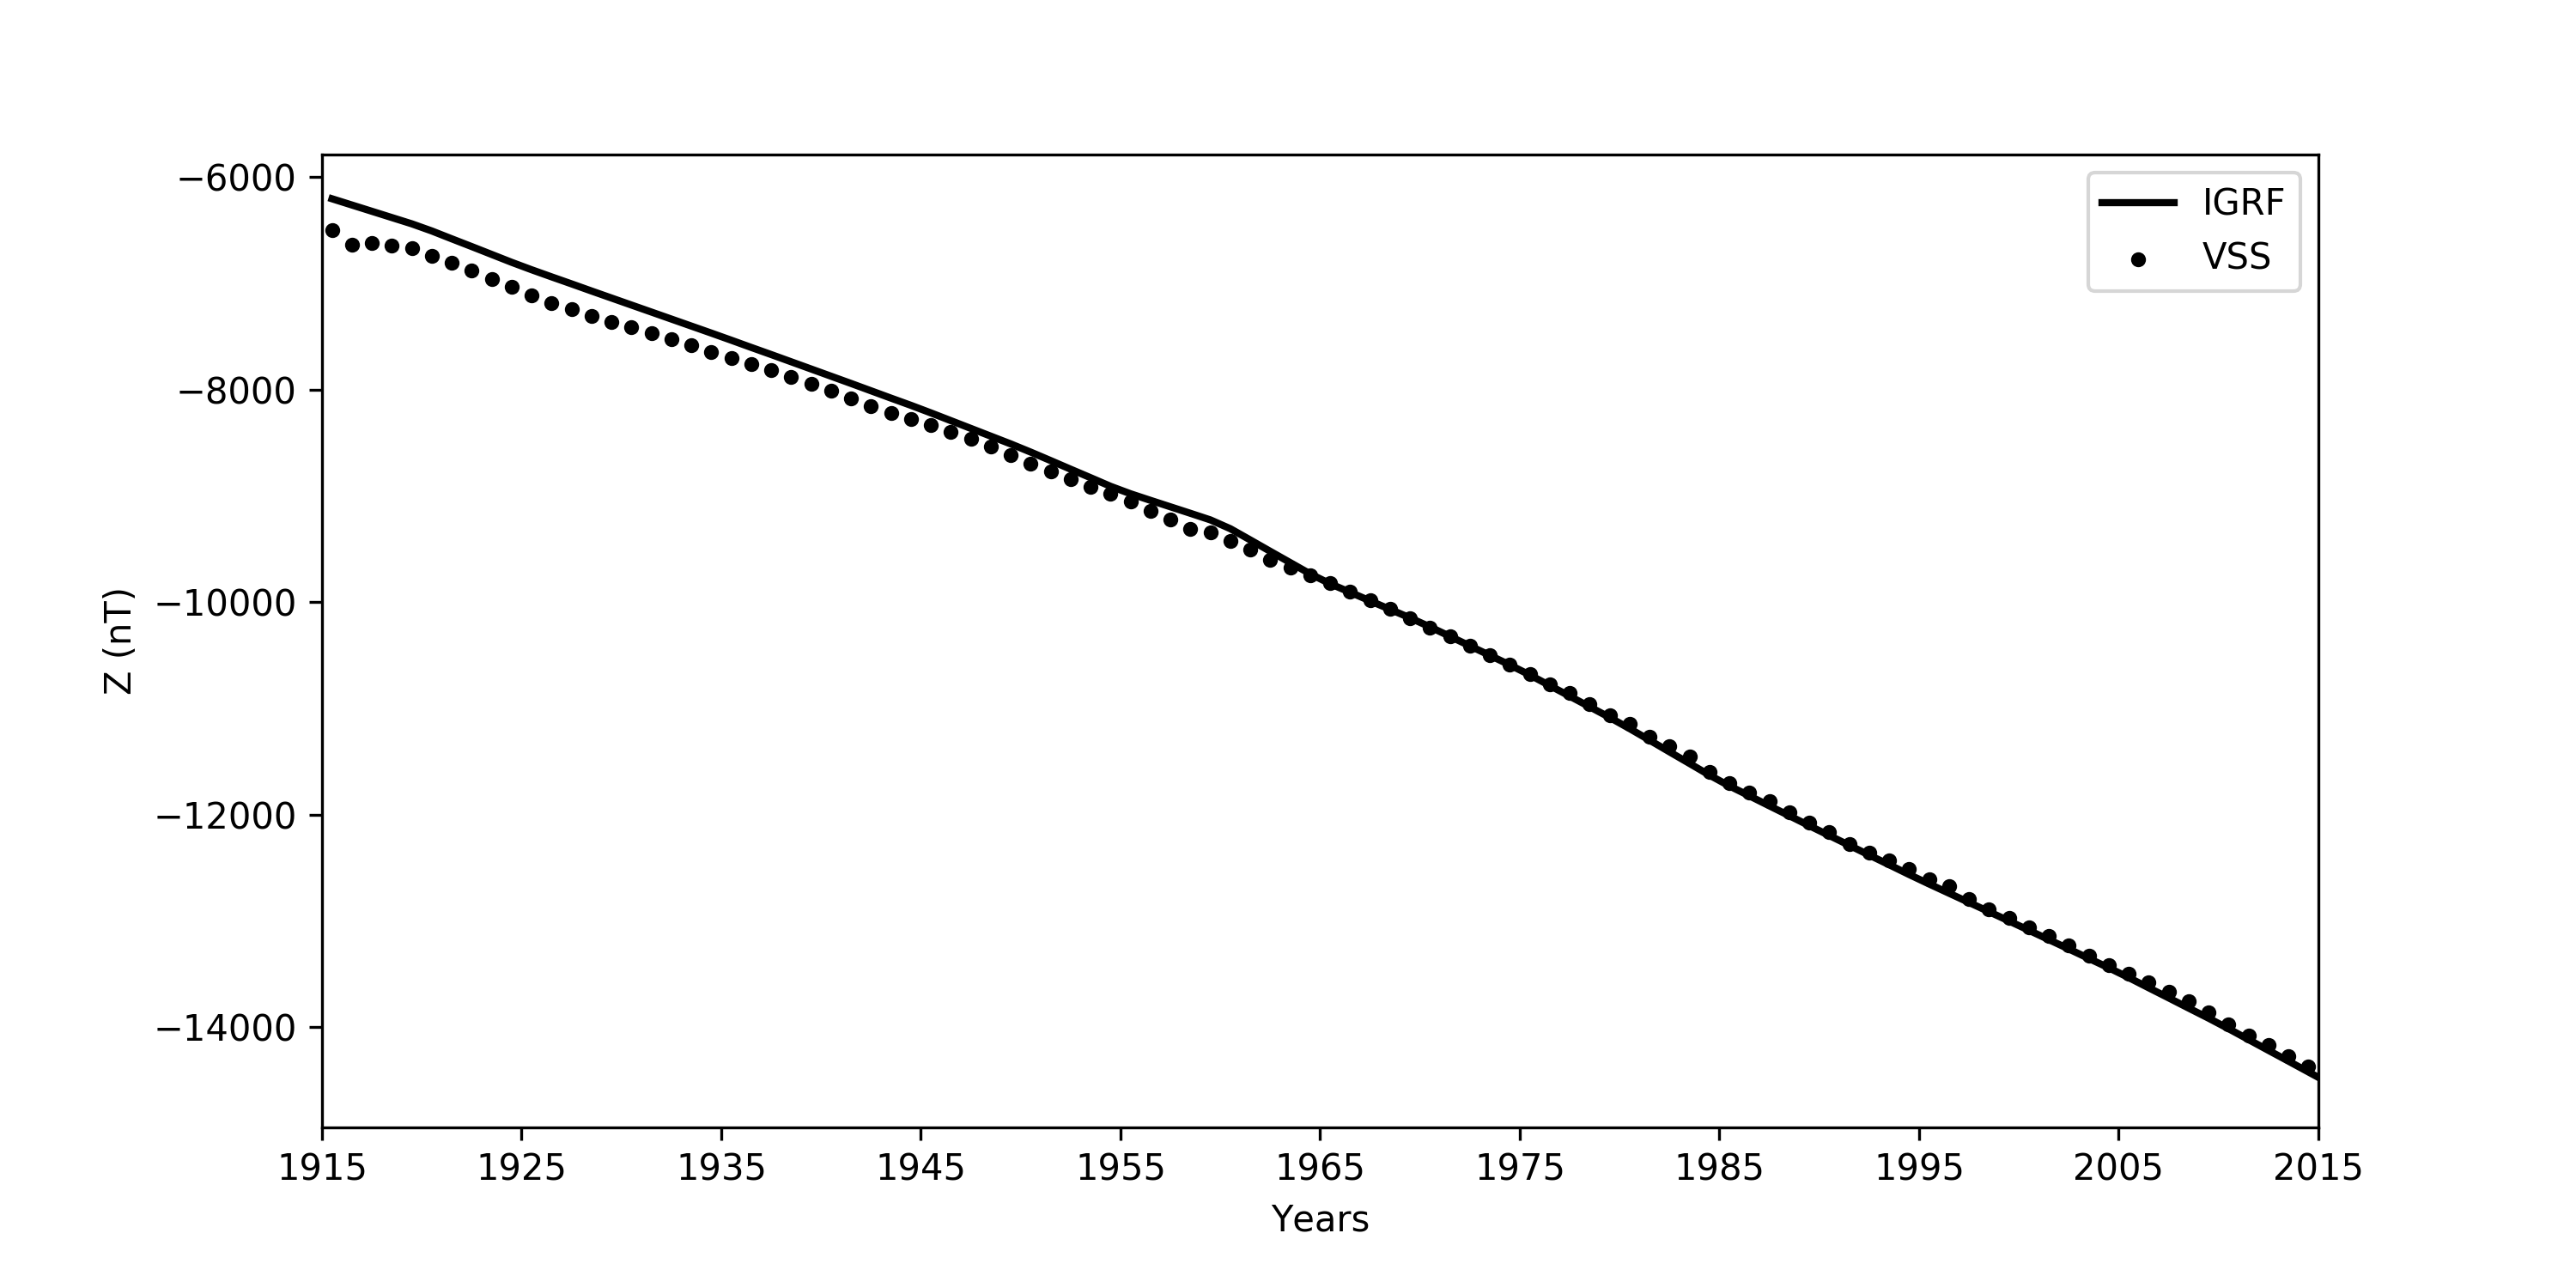
\includegraphics[width=1.0\linewidth]{Z}
%	\caption{3. RMS (Z component) = 1.22 (\%)}
%	\label{z}
%\end{figure}

%\begin{figure}
%	\centering
%	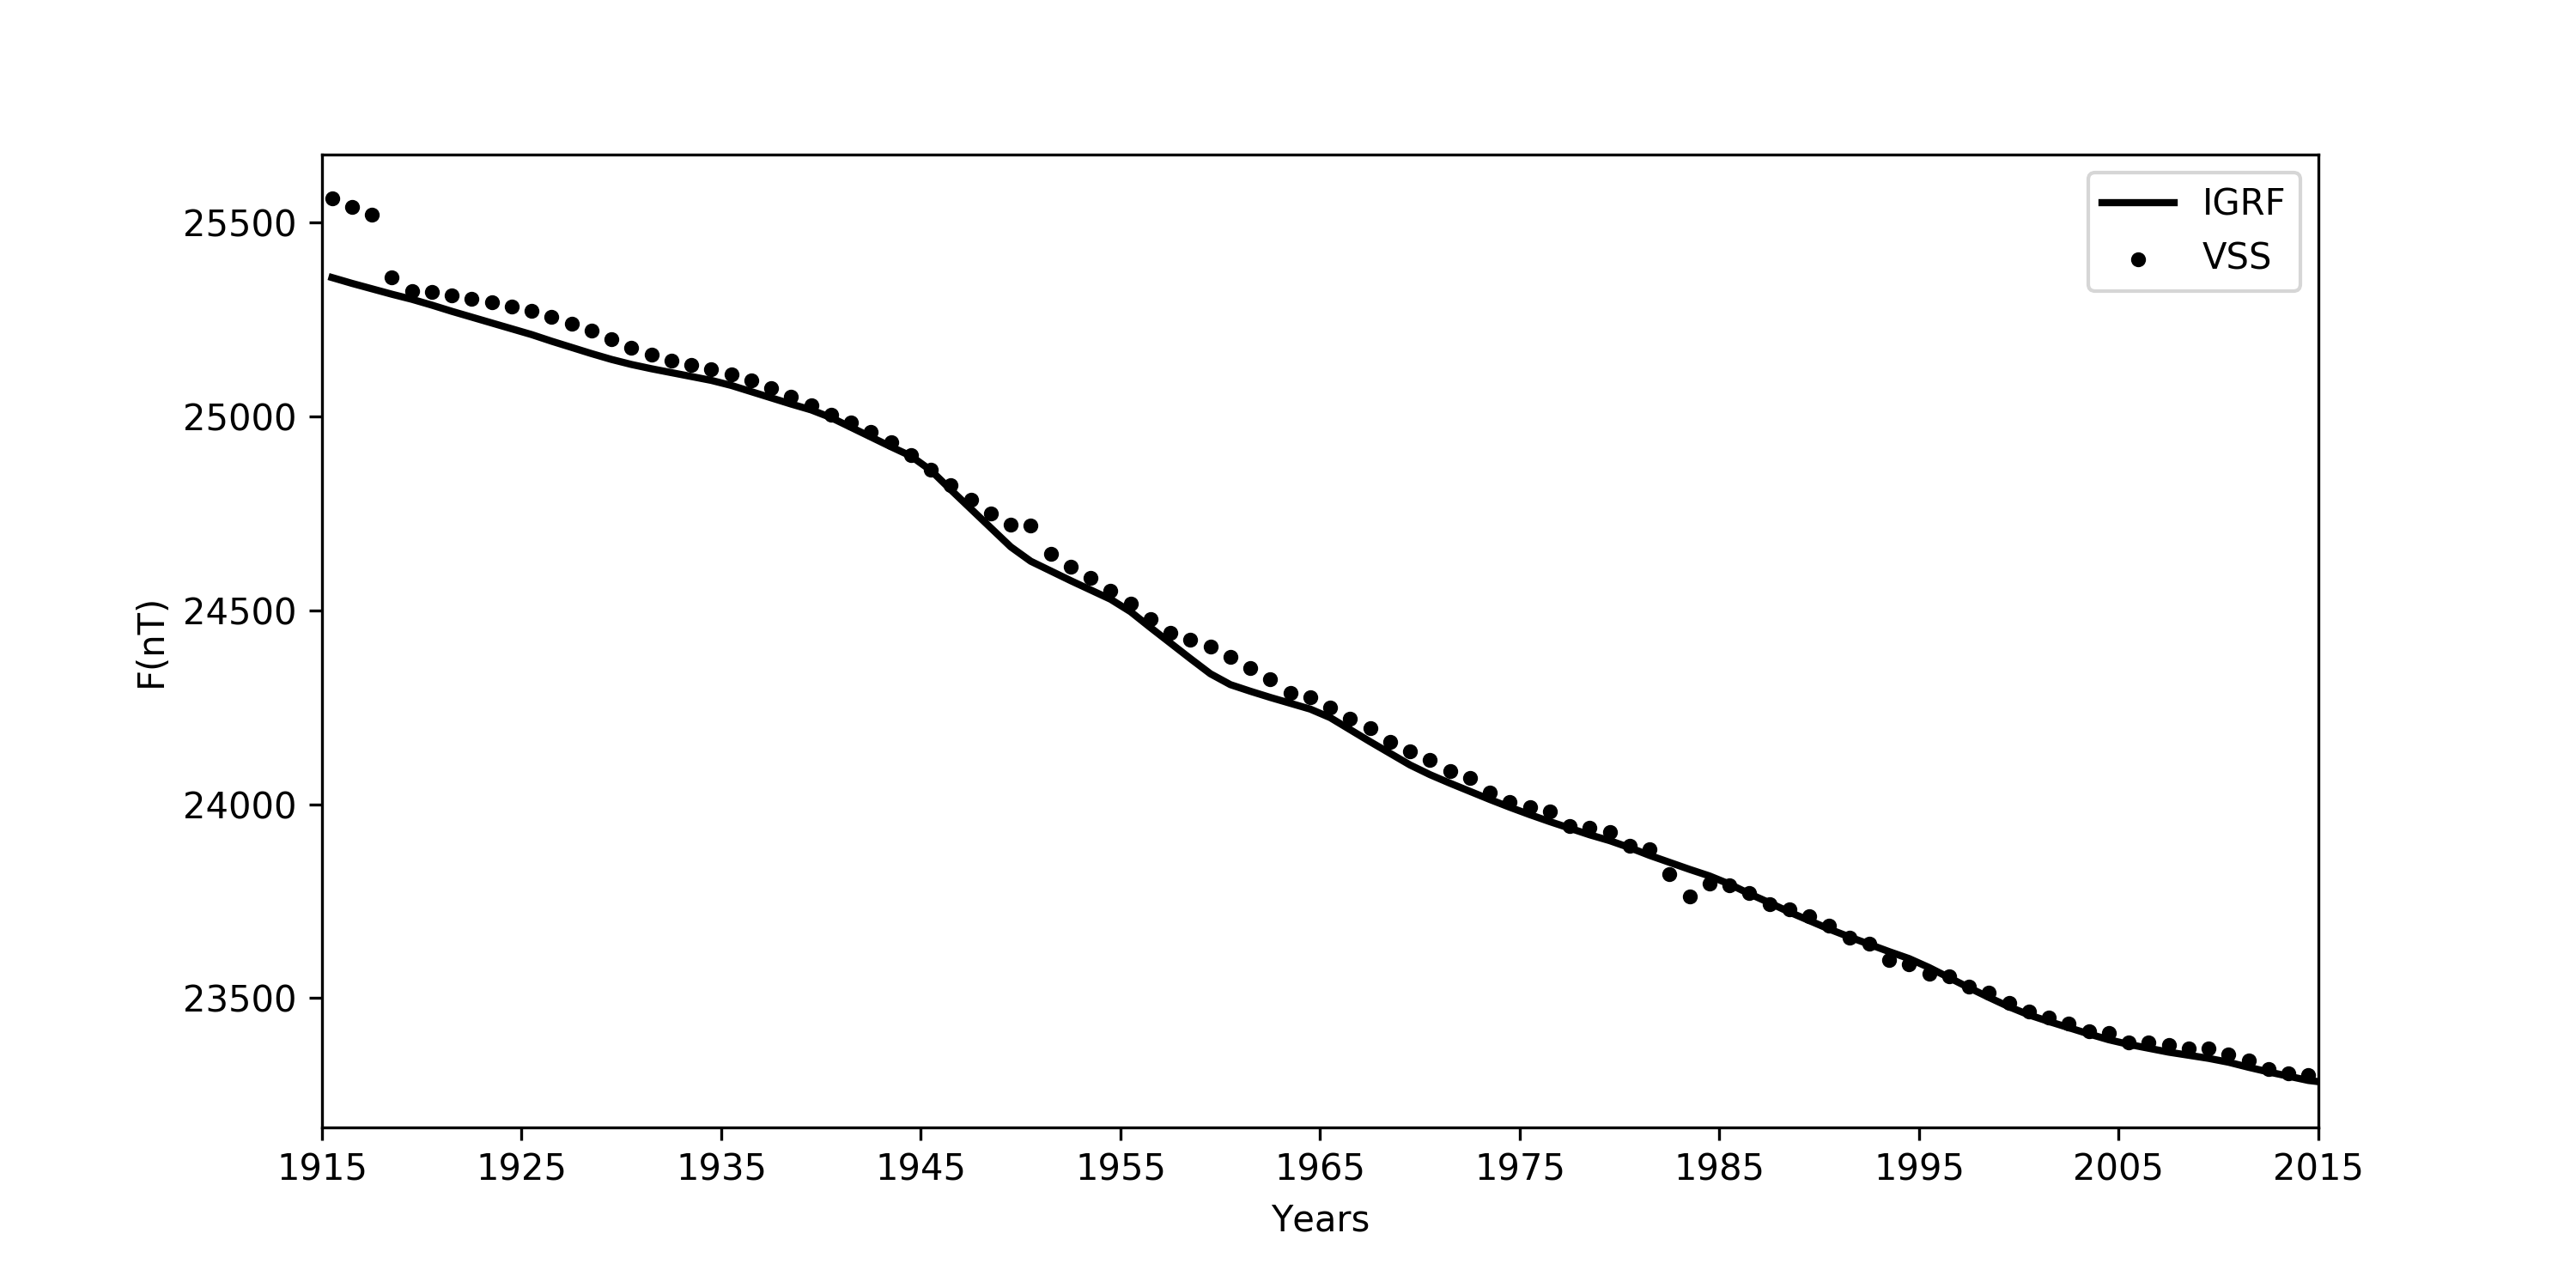
\includegraphics[width=1.0\linewidth]{F}
%	\caption{4. RMS (Intensity F) = 0.19 (\%)}
%	\label{f}
%\end{figure}



%\begin{figure}
%	\centering
%	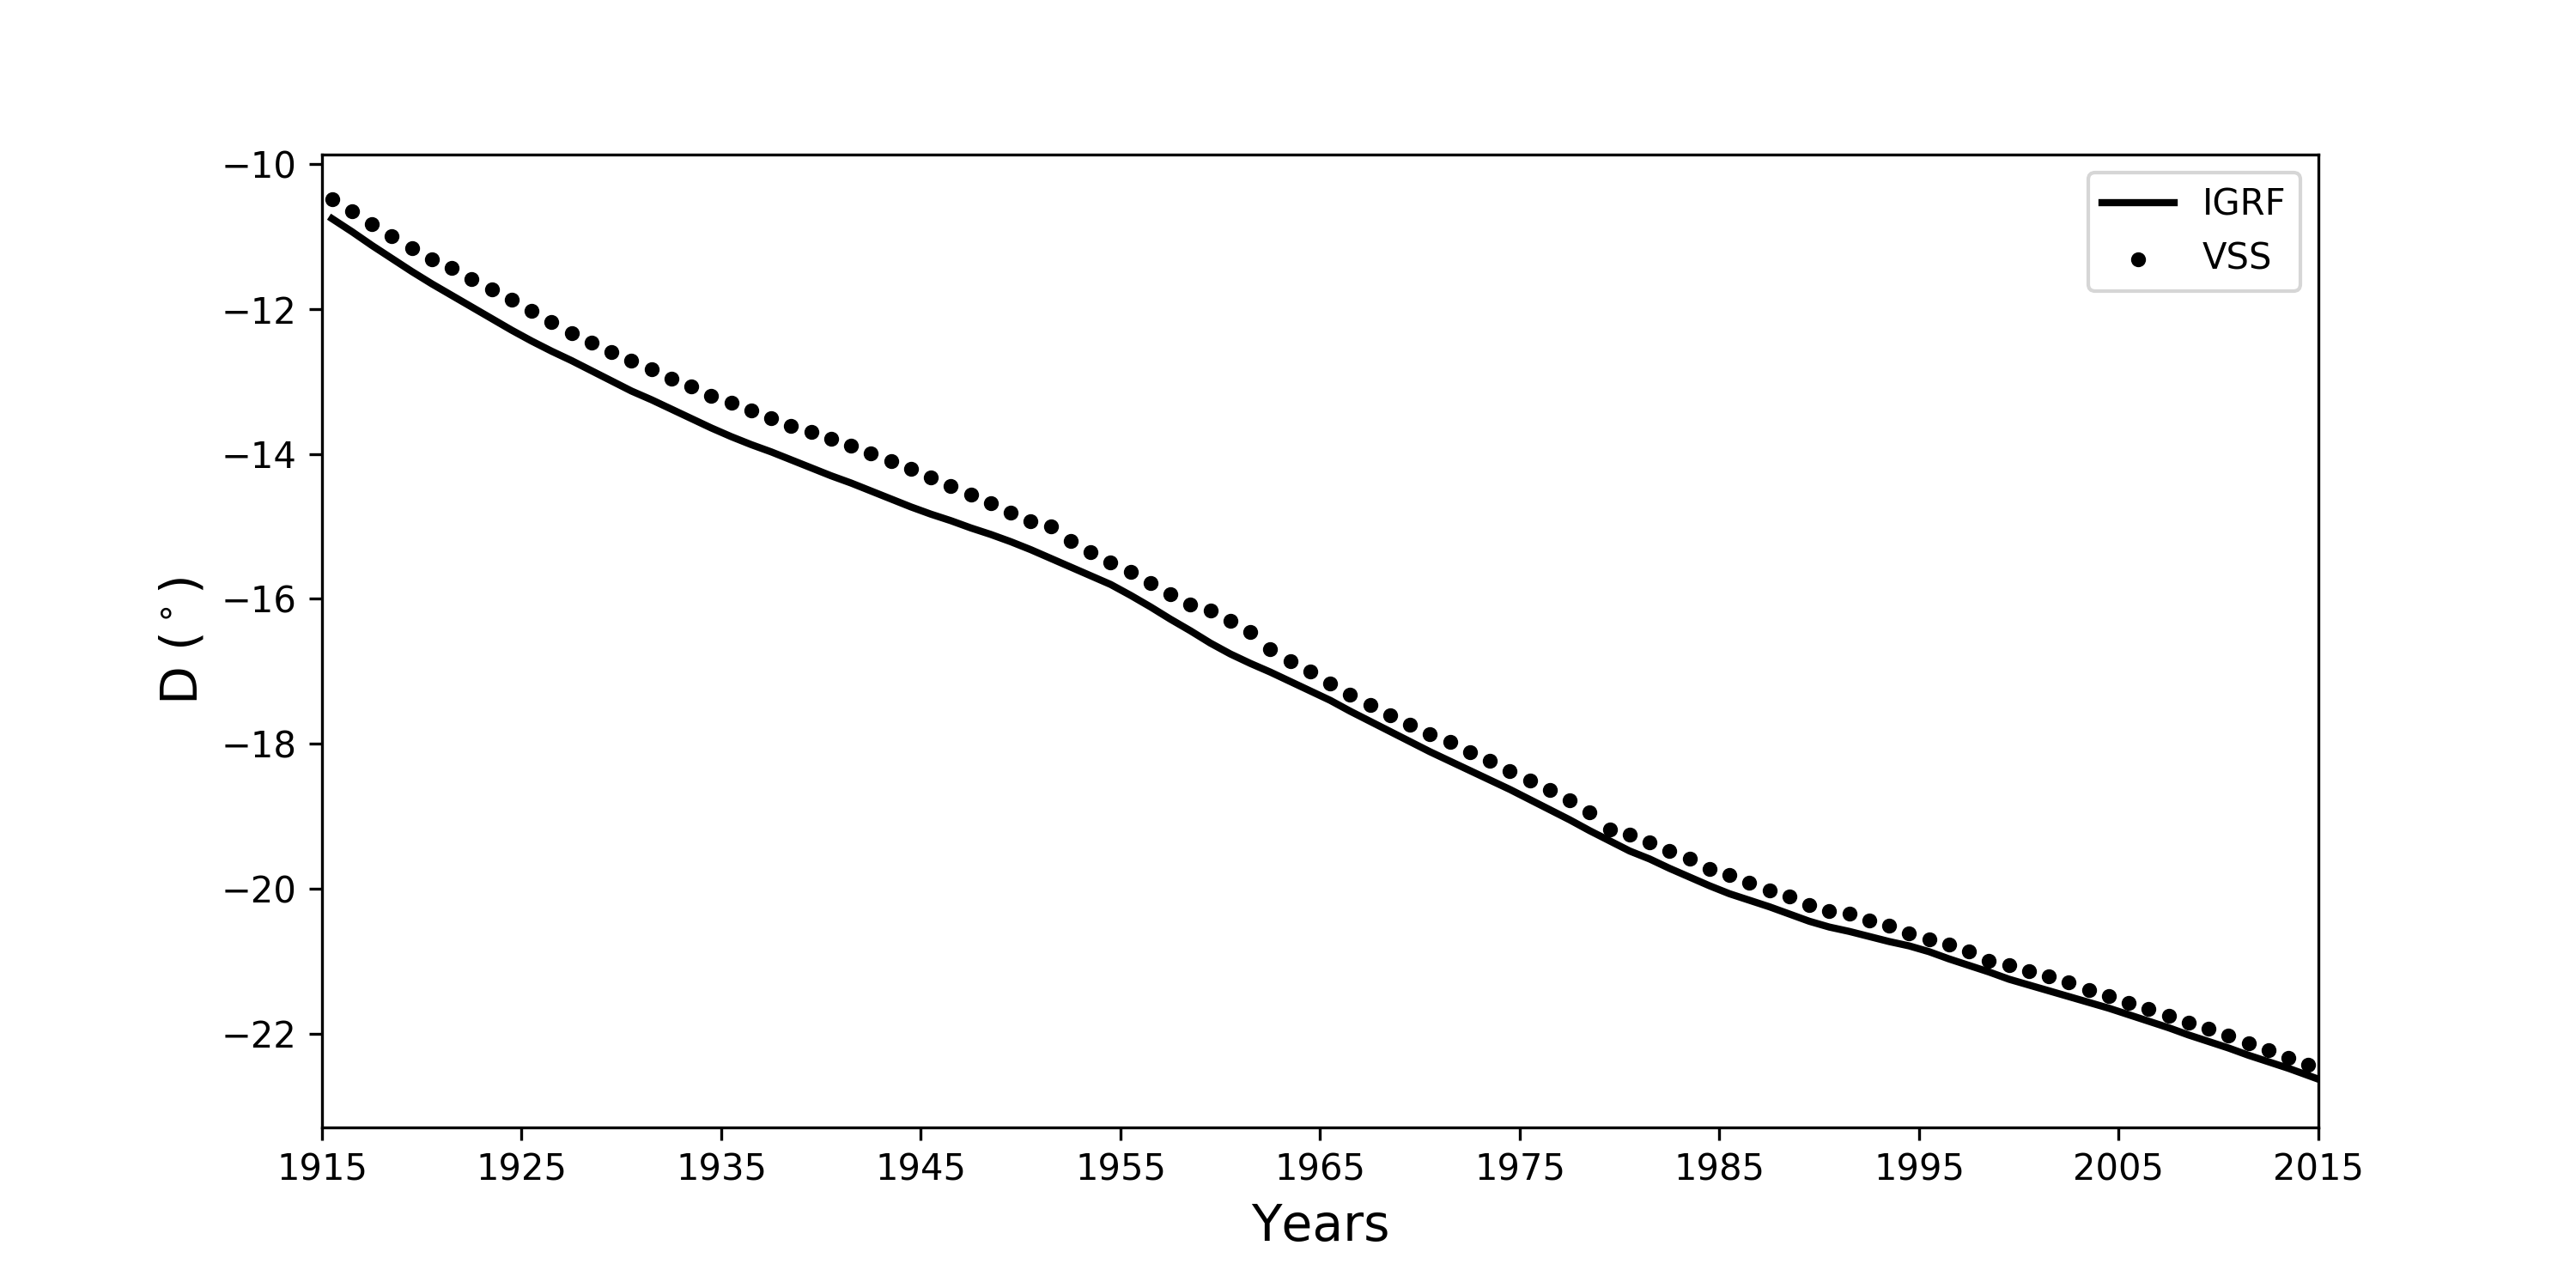
\includegraphics[width=1.0\linewidth]{D}
%	\caption{5. RMS (Inclination) = 1.1 (\%)}
%	\label{fo}
%\end{figure}


%\begin{figure}
%	\centering
%	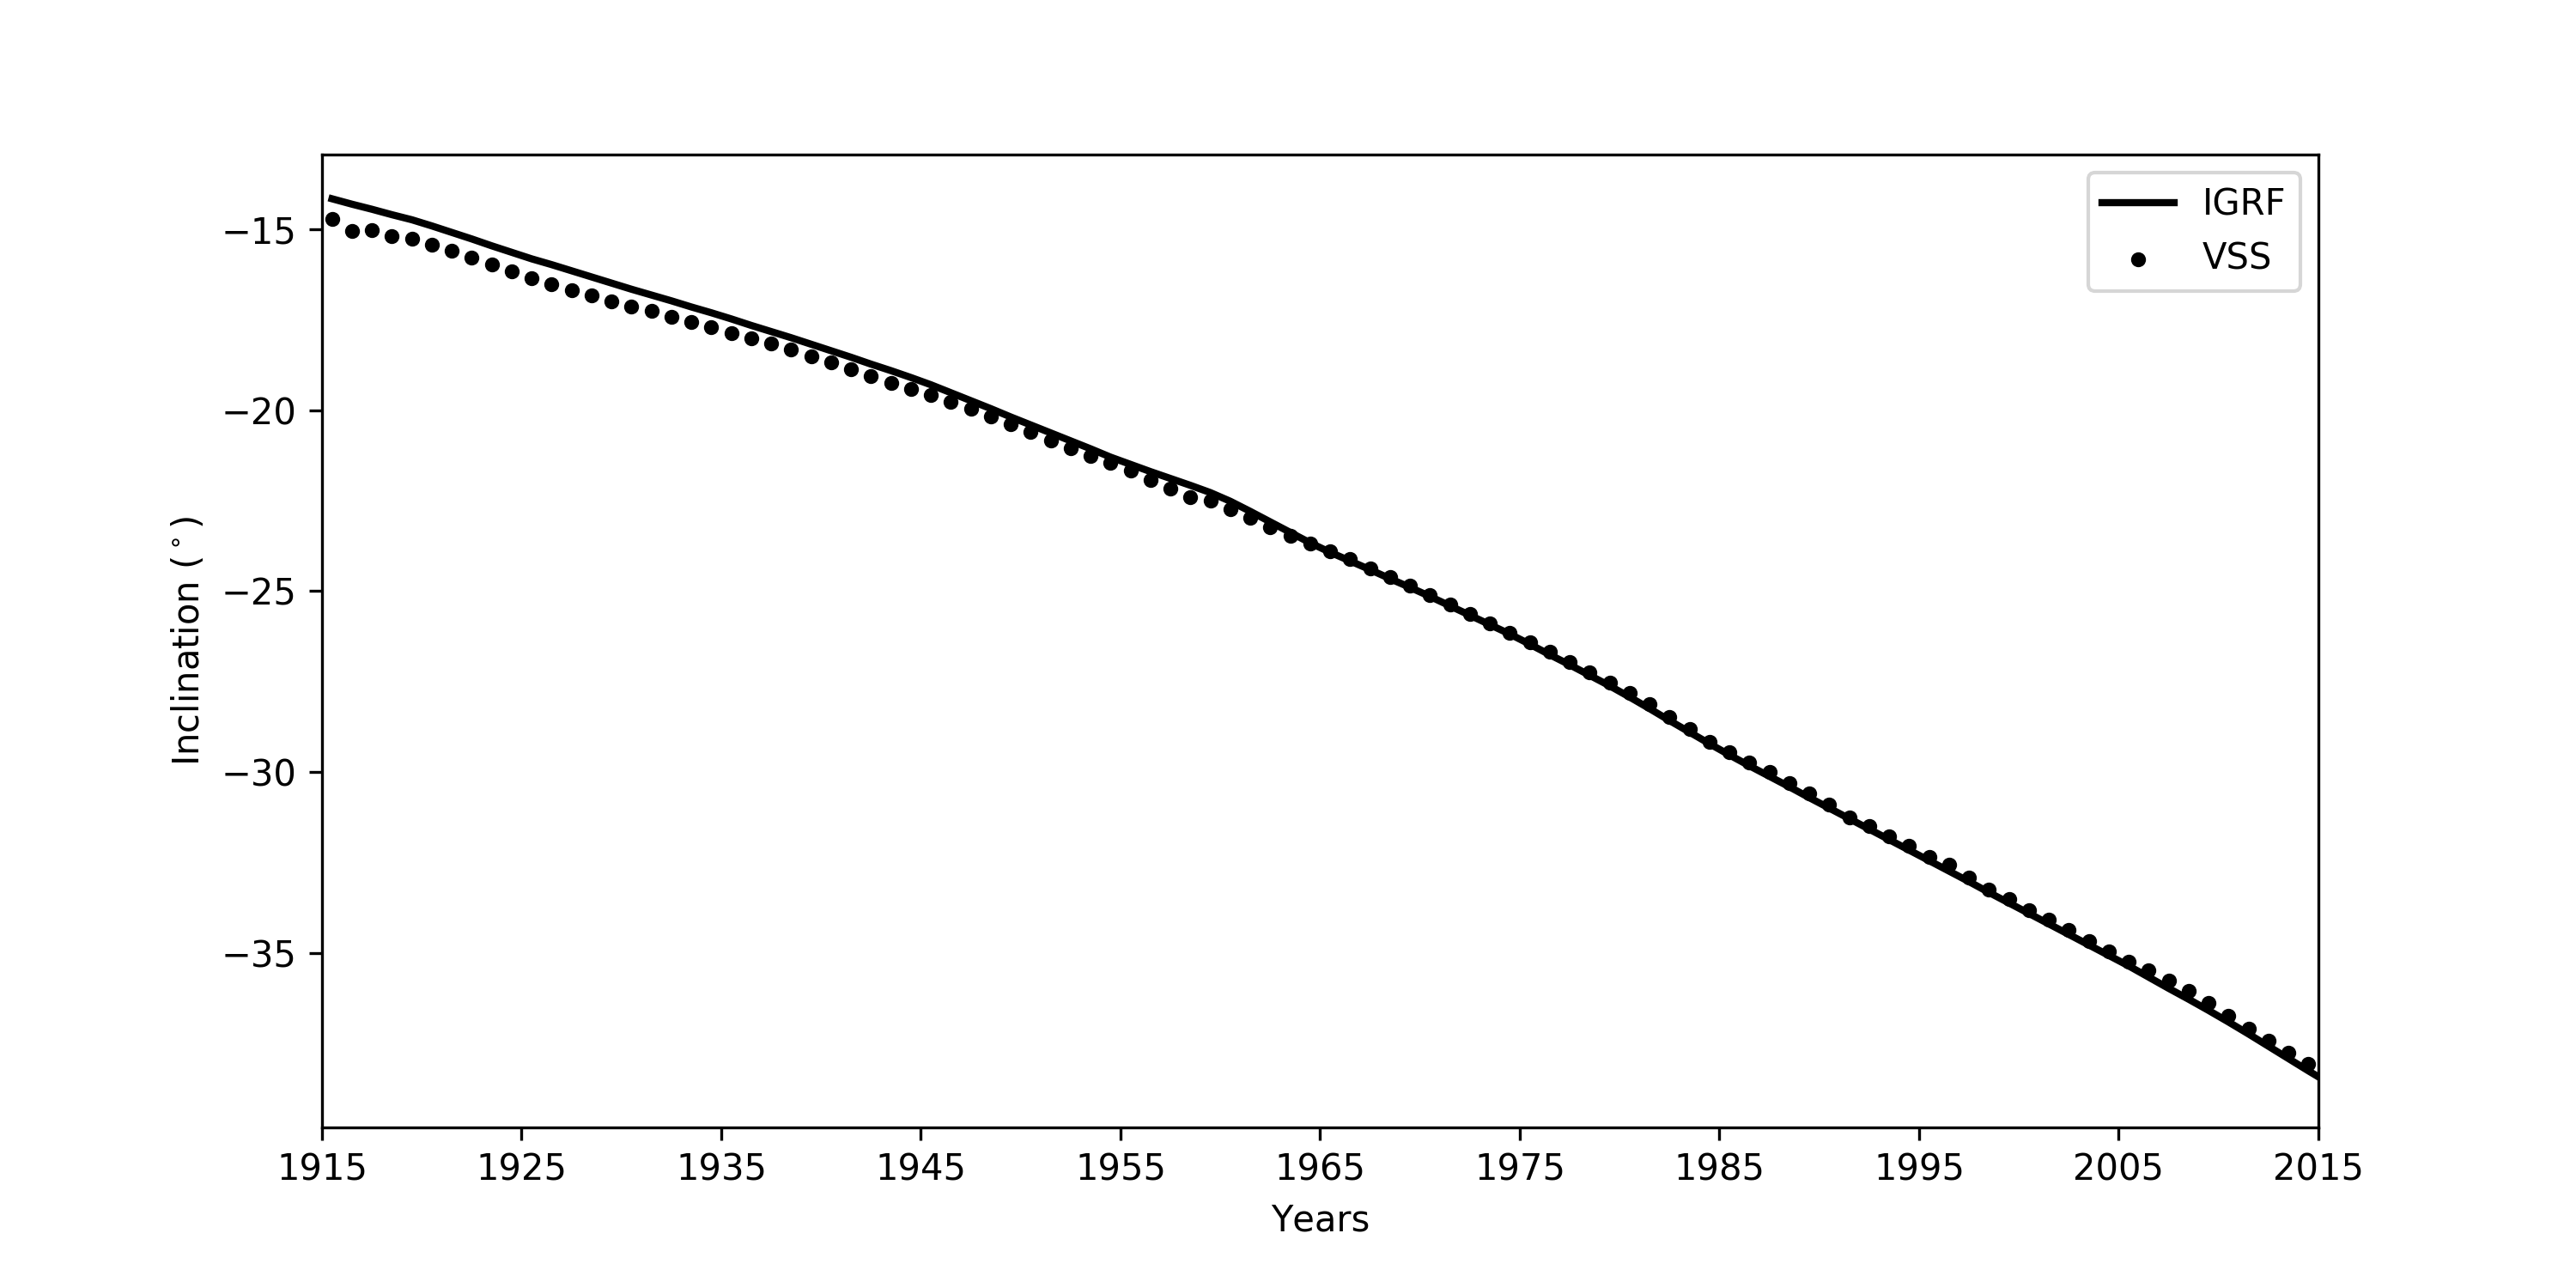
\includegraphics[width=1.0\linewidth]{I}
%	\caption{6. RMS (Declination) = 1.88 (\%)}
%	\label{ico}
%\end{figure}


%	\begin{figure}
%		\centering
%		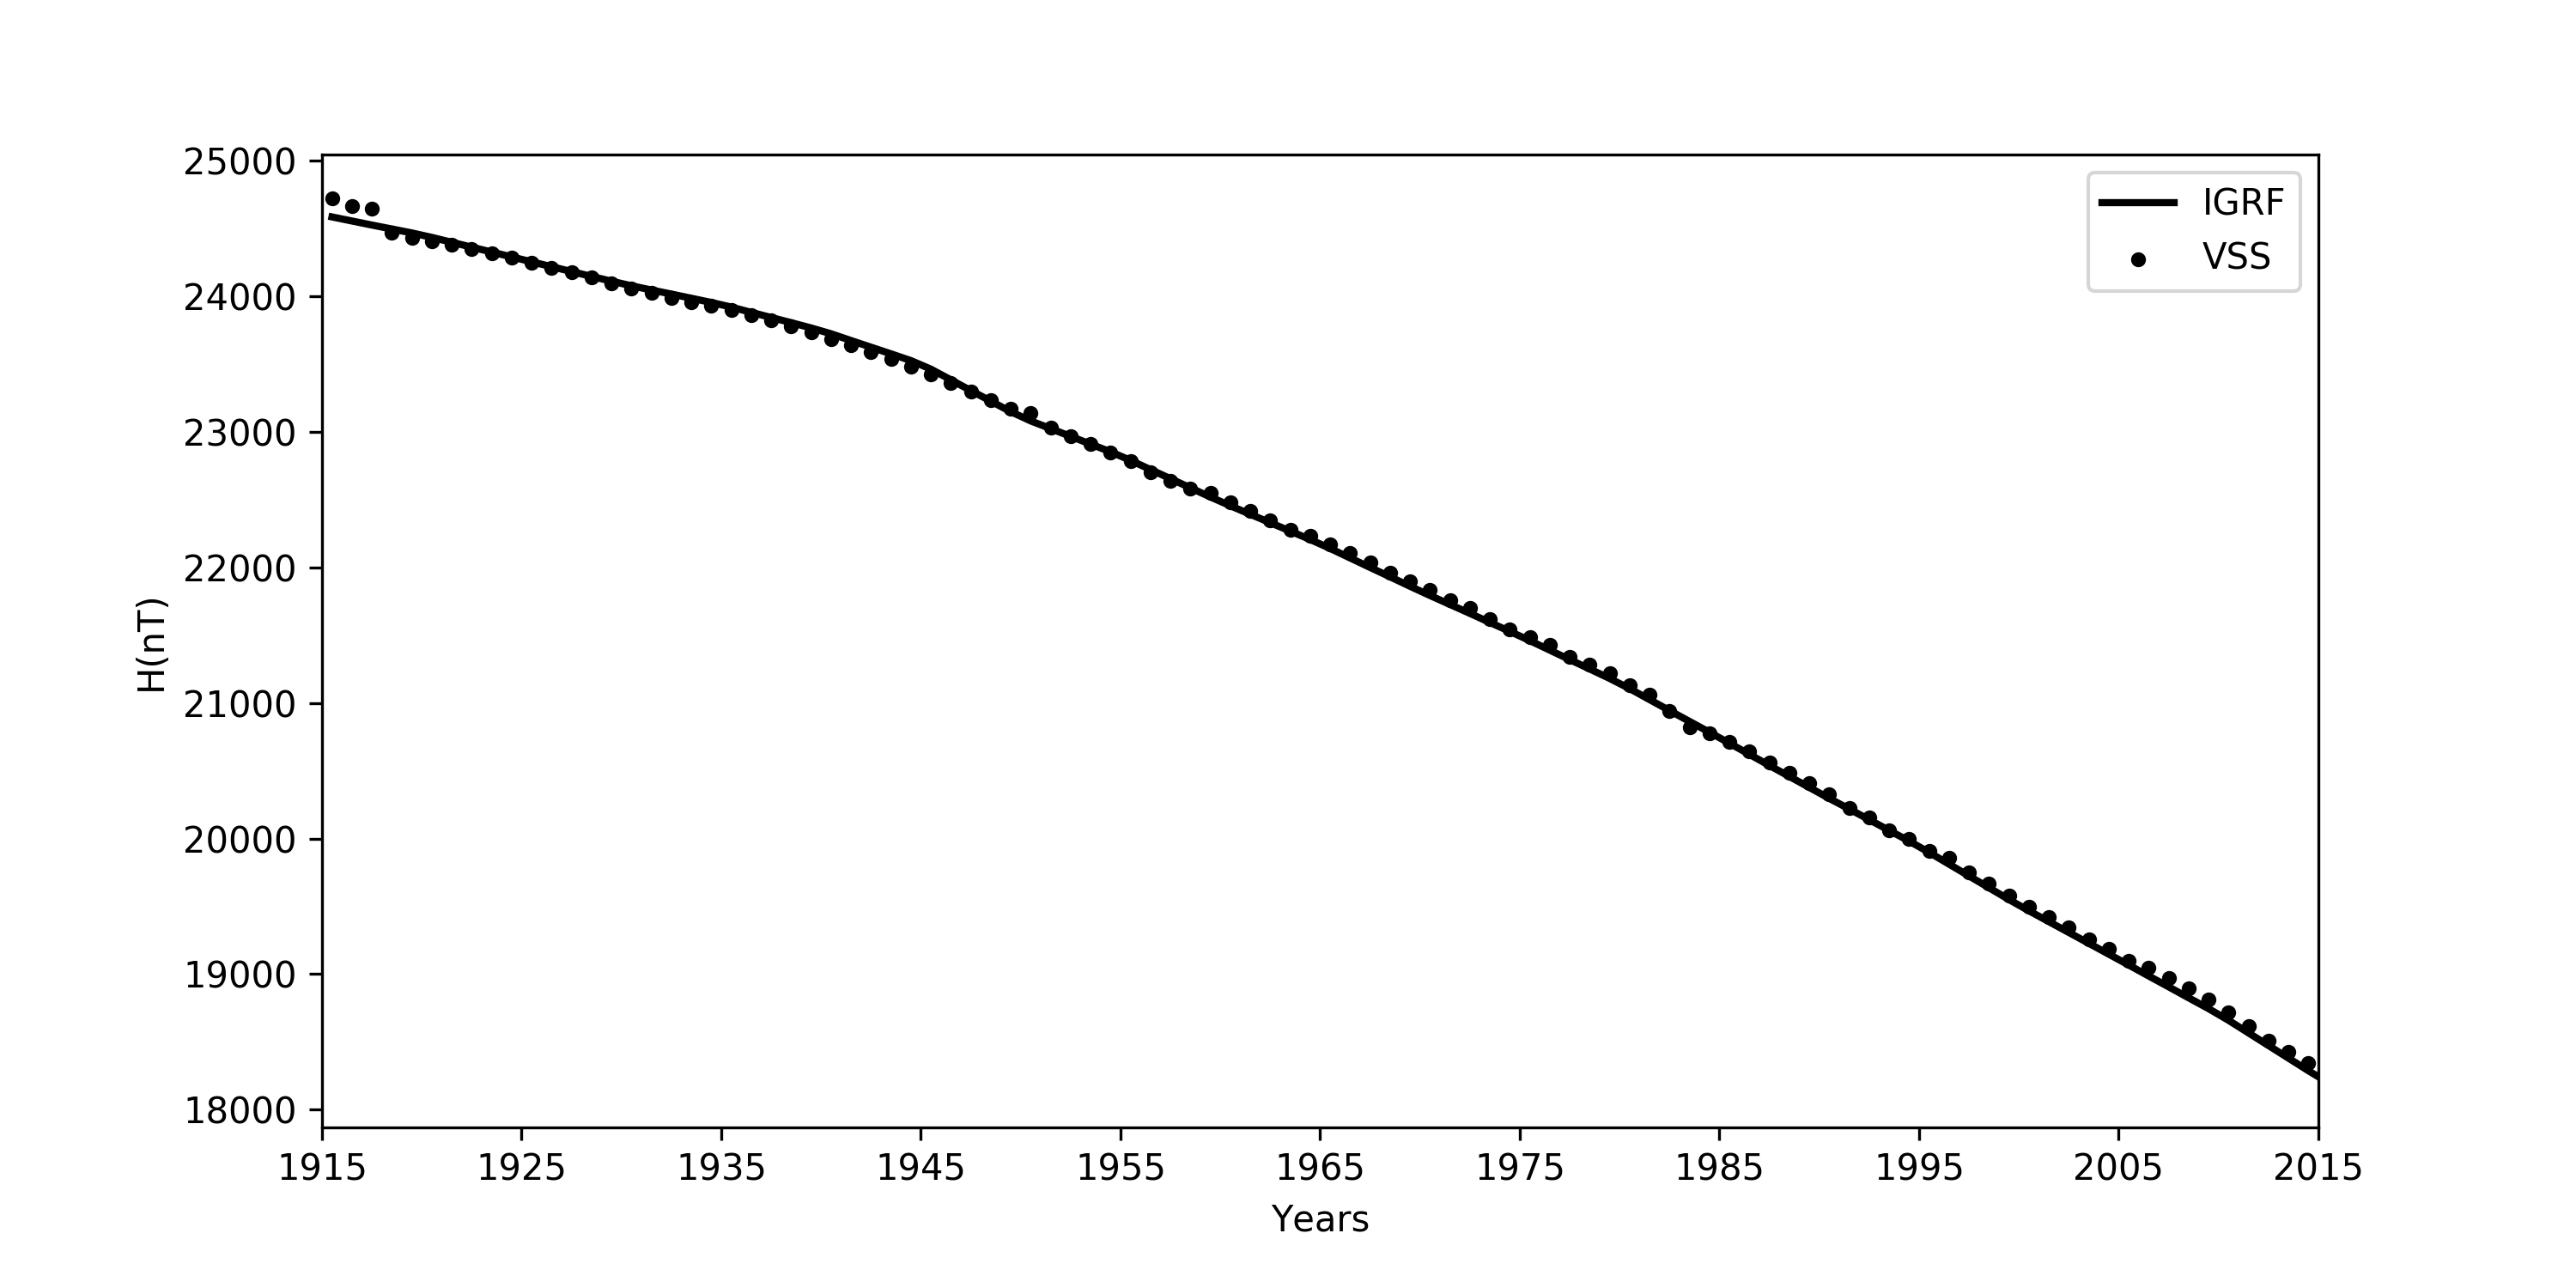
\includegraphics[width=1.0\linewidth]{H}
%		\caption{7. RMS (H component) = 1.98 (\%)}
%		\label{f_Sintetico}
%	\end{figure}

